\documentclass[conference]{IEEEtran}

\usepackage[utf8]{inputenc}
\usepackage{amsmath}
\usepackage{booktabs}
\usepackage{graphicx}
\usepackage{url}

\newcommand{\file}[1]{\path{#1}}
\emergencystretch=2em

\title{Virtual Memory Replacement \& Allocation: Efficiency--Fairness Trade-offs Under Memory Pressure}

\author{%
  Pranav Kumar Kaliaperumal, Akanksha Gutal, Spandana Erukulla\\
  Department of Computer Science and Engineering\\
  CSCI 5573: Operating Systems\\
  University of Colorado Denver\\
}

\begin{document}

\maketitle

\begin{abstract}
This report presents a custom virtual-memory simulator and trace-driven benchmarking framework for evaluating page replacement and frame allocation under multiprogrammed memory pressure. The simulator implements FIFO, LRU, NRU, Second Chance, and WSClock replacement with global, local, and proportional allocation. Across 1,005 aggregate configurations and 10,050 trial rows, the final campaign shows that fault-minimizing policies are not necessarily fairness-preserving policies. In the synthetic workload table, FIFO with global allocation produced the lowest mean page-fault counts for all four workload families, whereas NRU with local or proportional allocation minimized worst-case slowdown. The hypothesis evaluation supports H1 and H2: global allocation can reduce faults while increasing tail slowdown, and fairness variance increases near the aggregate working-set boundary. H3 is not supported; simple local policies did not improve the mixed-workload fairness condition tested. These results show that page-fault minimization alone is an incomplete criterion for policy selection under heterogeneous, fairness-sensitive workloads.
\end{abstract}

\section{Introduction}
Virtual memory is one of the core abstractions in operating systems: it separates the address space seen by a process from the limited physical frames available in the machine. Demand paging lets programs exceed physical memory capacity, but it also forces the operating system to decide which resident pages to evict and how many frames each process should receive. These decisions directly affect page-fault frequency, disk activity, runtime, and the quality of service received by competing processes.

This project connects directly to the operating-systems course topics of paging, page replacement, working sets, frame allocation, multiprogramming, and systems measurement. The course treatment explains the mechanisms; this report evaluates their interactions experimentally. In particular, it asks whether a policy that improves global efficiency can also hurt fairness when multiple processes compete near their aggregate working-set size (WSS).

Prior work established the theoretical importance of replacement choices and locality, including Belady's analysis of replacement algorithms and Denning's working-set model \cite{Belady1966,Denning1968,Denning1970}. Modern systems continue to revisit virtual-memory overheads, allocation behavior, and measurement sensitivity as machines grow in memory capacity and complexity \cite{Basu2013,Park2022,Powers2019,Mytkowicz2009}. Our contribution is a controlled framework that combines replacement policy, allocation policy, workload generation, trace replay, and fairness metrics in one reproducible evaluation.

The central claim is that replacement and allocation must be evaluated jointly: the policy combination that minimizes faults can differ from the combination that protects the slowest process under pressure.

The research questions were:
\begin{itemize}
  \item \textbf{RQ1:} Which replacement/allocation pairings reduce page faults without creating unfair slowdown across processes?
  \item \textbf{RQ2:} Does memory pressure near aggregate WSS create a threshold where global allocation stops helping fairness?
  \item \textbf{RQ3:} Can simpler local policies such as FIFO or NRU outperform history-based global policies on fairness for heterogeneous workloads?
\end{itemize}

\textbf{Contributions.} This project makes the following contributions:
\begin{enumerate}
  \item A custom Python-based virtual memory simulator with trace-driven replay support.
  \item A benchmarking framework covering five replacement algorithms and three allocation policies.
  \item A repeated experimental study across synthetic and trace-driven workloads under controlled memory pressure.
  \item An efficiency--fairness analysis showing that fault reduction and slowdown fairness can diverge near the working-set boundary.
  \item A reproducible artifact bundle containing processed results, figures, tables, and demo materials.
\end{enumerate}

\section{Relationship to Operating Systems}
Virtual memory is a major operating-system service. It hides the limited size of physical memory, enables multiprogramming, and provides isolation between processes. Page replacement and frame allocation are core memory-management topics that appear in every undergraduate and graduate operating-systems curriculum \cite{Silberschatz2019}. The operating system must decide which pages to keep resident and how many frames each process deserves; these decisions directly influence throughput, response time, and the risk of thrashing.

This project studies multiprogramming interference, memory pressure, fairness, and system efficiency---all themes that are central to the course. The course lectures explain FIFO, LRU, NRU, Second Chance, and WSClock replacement, together with global, local, and proportional allocation strategies. The course also introduces the working-set model and thrashing. This report takes those classroom concepts and evaluates them in a controlled simulator, making the abstract trade-offs concrete. By measuring both efficiency (page faults, disk activity) and fairness (slowdown, Jain's index), the project mirrors the real-world tension that operating-system designers face: a policy that minimizes global faults may still disadvantage individual processes.

The connection is therefore not merely thematic. The simulator implements the algorithms discussed in the course, the workloads stress the memory-pressure conditions associated with thrashing, and the fairness metrics quantify the ``quality of service'' concern that arises when multiple processes compete for memory.

\section{Related Work}
Belady's study of virtual-storage replacement algorithms showed that simple eviction policies can behave pathologically, including FIFO cases where adding frames can increase faults \cite{Belady1966}. Denning's working-set model then connected paging behavior to locality by arguing that a process has a time-varying set of pages that must remain resident to avoid excessive faults \cite{Denning1968}. Denning's later survey placed these ideas in the broader design space of virtual memory mechanisms and adaptive policy choices \cite{Denning1970}. These classical papers remain the conceptual foundation for modern memory management.

Frame allocation is the second half of the paging decision. Operating systems texts distinguish local replacement, where each process competes mainly with its own resident set, from global replacement, where processes compete for a shared pool of frames \cite{Silberschatz2019}. Proportional allocation adds a compromise by dividing frames according to process demand. Ghandeharizadeh et al. studied cache replacement with explicit memory allocation as a joint optimization problem rather than as replacement alone \cite{Ghandeharizadeh2015}. Their work shows that treating cache size as a decision variable---just as we treat frame allocation---can yield better combined performance than optimizing replacement in isolation.

Modern systems keep virtual memory relevant because page tables, memory allocators, and compaction layers all create measurable overheads at scale. Basu et al. studied efficient virtual memory for large-memory servers, showing that TLB misses and page-table walks can consume a significant fraction of execution time \cite{Basu2013}. Park et al. examined page-table caching pressure and proposed flattening and cache prioritization to reduce walk latency \cite{Park2022}. Schwalb et al. addressed persistent-memory allocation, demonstrating that NVRAM allocators must balance wear leveling with fragmentation \cite{Schwalb2015}. Powers et al. explored memory compaction for C/C++ programs, breaking classical Robson bounds by meshing pages without relocation \cite{Powers2019}. These works motivate why the replacement/allocation boundary remains important beyond textbook examples.

This report differs from prior work by focusing on a course-scale but end-to-end empirical framework. It does not propose a new kernel policy. Instead, it contributes a transparent simulator and artifact bundle that make the efficiency-versus-fairness trade-off visible across replacement policy, allocation policy, memory pressure, synthetic workload family, and trace-driven replay. The classical studies provide theoretical grounding; the modern studies provide motivation. Our work bridges the two by offering a reproducible teaching-scale platform for experimental evaluation.

\section{System Design and Implementation}
The project is implemented as a custom Python-based simulator rather than as a production-kernel modification. The simulator models page accesses, page tables, physical frames, replacement decisions, allocation boundaries, and per-process accounting. Its design has four main components.

\textbf{Workload generator.} The workload generator constructs synthetic memory-reference streams for high-locality, streaming, mixed, and thrashing workloads. These families stress different access behaviors: compact reuse, sequential scans, heterogeneous mixes, and pressure-heavy fault patterns. The generator is parameterized by working-set size, sequence length, and locality strength so that experiments can sweep memory pressure systematically. The same interface also accepts normalized trace events loaded from CSV files under \file{workloads/traces/}, enabling replay of concrete reference streams alongside synthetic families.

\textbf{Memory manager.} The memory manager maintains per-process page tables and a configurable physical-frame pool. It supports \texttt{GlobalAllocation}, \texttt{LocalAllocation}, and \texttt{ProportionalAllocation}. Global allocation lets processes compete for a shared frame pool; local allocation isolates each process more strongly by reserving a fixed partition; proportional allocation divides memory according to estimated demand so that larger working sets receive larger shares. The manager records every page fault, replacement, disk read, disk write, and replacement event in per-process logs.

\textbf{Policy engine.} The policy engine implements FIFO, LRU, NRU, Second Chance, and WSClock. These policies cover a range from simple insertion-order eviction to reference-bit approximations and working-set-inspired clock behavior. Each policy exposes a common interface---\texttt{select\_victim(frame\_pool, process\_id)}---so the experiment runner can vary replacement and allocation independently without changing the core simulator loop. FIFO and LRU use list-based state; NRU uses a reference bit sampled at fixed intervals; Second Chance uses a circular queue with a second-chance bit; WSClock combines a clock hand with an age threshold based on the working-set window $\tau$.

\textbf{Experiment and analysis layer.} The experiment layer automates repeated runs, exports JSON/CSV summaries, computes slowdown from isolated and shared runtimes, validates processed outputs, and generates report tables and figures. The primary entry points are \file{main.py}, \file{experiments/run\_all\_experiments.py}, \file{scripts/aggregate\_final\_results.py}, \file{scripts/validate\_results.py}, \file{scripts/build\_report\_tables.py}, and \file{scripts/build\_report\_figures.py}. Windows and Unix wrapper scripts provide quiet-run and pinned-core execution paths for more stable timing metadata.

\textbf{Trace-driven replay.} The trace-driven component reads pre-recorded reference strings from CSV files, normalizes page numbers to a per-process namespace, and replays them through the same memory manager used for synthetic workloads. This ensures that trace-driven and synthetic results are directly comparable: the only difference is the source of the reference string, not the replacement or allocation logic.

\section{Experimental Methodology}
The final campaign used the locked raw campaign \file{results/raw/campaign\_20260404\_140330\_266}. Table~\ref{tab:matrix_scope} summarizes the report-grade scope. The synthetic matrix used five replacement algorithms, three allocation policies, four workload families, four memory-pressure levels, three process counts, and ten repetitions. The trace-driven side used five checked-in report traces; trace rows preserve the process counts encoded in the trace rather than forcing the synthetic 2/4/8 grid.

\begin{table}[t]
\centering
\footnotesize
\caption{Final campaign scope.}
\label{tab:matrix_scope}
\begin{tabular}{@{}p{0.30\linewidth}p{0.58\linewidth}@{}}
\toprule
Factor & Final setting \\
\midrule
Replacement algorithms & FIFO, LRU, NRU, Second Chance, WSClock \\
Allocation policies & GlobalAllocation, LocalAllocation, ProportionalAllocation \\
Synthetic workloads & high\_locality, streaming, mixed, thrashing \\
Memory levels & 0.8x, 1.0x, 1.2x, 1.5x aggregate WSS \\
Synthetic process counts & 2, 4, 8 \\
Repetitions & 10 per synthetic configuration \\
Report-grade aggregate & 1005 configuration groups / 10,050 trial rows \\
Trace families & Five report traces: report\_locality\_heavy, report\_mixed\_heterogeneous, report\_streaming\_sequential, report\_thrashing\_pressure, and sample\_trace \\
\bottomrule
\end{tabular}
\end{table}

The memory-pressure settings were defined relative to aggregate WSS. This makes the experiments comparable across workloads with different locality footprints. At 1.5x WSS, the system has more slack; at 1.2x and 1.0x, it approaches the working-set boundary; at 0.8x, it operates under strong pressure.

Experiments were run on a Windows host with a 12th Gen Intel Core i5-12400F processor, 16 GB of RAM, and an NVIDIA RTX 3050 GPU. Runtime-sensitive experiments used wrapper scripts such as \file{scripts/run\_quiet\_benchmark.ps1} and \file{scripts/run\_pinned.ps1} to capture environment metadata and reduce host interference. These controls improve repeatability, but they do not eliminate all wall-clock noise.

\section{Metrics, Repetition, and Statistical Treatment}
The simulator records page faults, page replacements, disk reads, disk writes, total disk activity, and runtime-derived slowdown. Page faults and disk events represent efficiency. Slowdown is measured by running each workload both in isolation and in a shared multiprogrammed setting, then computing
\[
\mathrm{slowdown} = \frac{t_{\mathrm{shared}}}{t_{\mathrm{isolated}}}.
\]
Fairness is summarized with worst-case slowdown, slowdown variance, coefficient of variation (CV), and Jain's fairness index. Jain's index is close to 1.0 when normalized performance is evenly distributed and lower when one or more processes receive worse service.

\textbf{Repetition and confidence.} Each aggregate configuration contains ten trial rows. From these repetitions we compute means, standard deviations, and 95\% confidence intervals for page-fault counts and fairness metrics. The hypothesis table is generated from \file{results/processed/hypothesis\_evaluation.csv}, while the report-facing policy tables are generated from \file{results/processed/final\_aggregate\_results.csv}. The refreshed validation bundle \file{results/processed/validation\_report.json} records 1,005 valid source groups, no duplicate source or configuration records, and zero missing shared or isolation runtime-record issues. Its remaining warnings are host-noise outliers, so page-fault trends and policy-rank patterns are more stable than exact wall-clock slowdown point estimates.

\textbf{Statistical treatment.} Because slowdown depends on wall-clock timing and is somewhat noisy, we treat slowdown directionally rather than as exact magnitudes. Page-fault counts and fairness-pattern trends (which allocation wins, which replacement wins) are more stable across repetitions and are therefore used as the primary signals for hypothesis evaluation. Conclusions are strongest for comparative trends, not for universal policy rankings.

\section{Results and Analysis}
\subsection{Campaign Coverage}
The final processed outputs are anchored by \file{results/processed/final\_aggregate\_results.csv}, \file{results/processed/hypothesis\_evaluation.csv}, and \file{results/processed/validation\_report.json}. The report-facing tables in \file{results/tables/} and figures in \file{results/figures/} were generated from these processed outputs. The campaign covers 720 synthetic aggregate configurations with 7,200 trials and 285 trace aggregate configurations with 2,850 trials. This lets us compare controlled stress patterns against concrete reference streams.

All quantitative findings in this report are drawn from the locked campaign outputs under \file{results/raw/campaign\_20260404\_140330\_266} and the processed summaries in \file{results/processed/final\_aggregate\_results.csv}, \file{results/processed/hypothesis\_evaluation.csv}, and \file{results/processed/validation\_report.json}. These files were regenerated and validated through the final artifact-build and smoke-test pipeline before report compilation.

\subsection{Synthetic Workload Results}
Table~\ref{tab:synthetic_best} reports the table-selected best policy combination for each synthetic workload under three metrics; ties are possible in the underlying aggregate. FIFO with global allocation produced the lowest mean page-fault counts across all four synthetic workload families. The fairness-oriented winners were different: NRU with proportional or local allocation minimized worst-case slowdown, and the highest Jain's-index winners came from local or proportional allocation. This split is the main empirical signal behind the paper: one policy pairing may reduce faults while another better protects the slowest process.

\begin{table}[t]
\centering
\small
\caption{Headline results by synthetic workload.}
\label{tab:synthetic_best}
\resizebox{\linewidth}{!}{%
\begin{tabular}{llll}
\toprule
Workload & Lowest page faults & Lowest worst slowdown & Highest Jain's index \\
\midrule
high\_locality & FIFO + GlobalAllocation (144.0) & NRU + ProportionalAllocation (1.5105) & SecondChance + LocalAllocation (0.99997) \\
mixed & FIFO + GlobalAllocation (202.7) & NRU + LocalAllocation (1.5054) & FIFO + LocalAllocation (0.99988) \\
streaming & FIFO + GlobalAllocation (340.0) & NRU + LocalAllocation (1.4488) & LRU + ProportionalAllocation (0.99991) \\
thrashing & FIFO + GlobalAllocation (204.0) & NRU + ProportionalAllocation (1.5057) & FIFO + LocalAllocation (0.99987) \\
\bottomrule
\end{tabular}%
}
\end{table}

\begin{figure}[t]
\centering
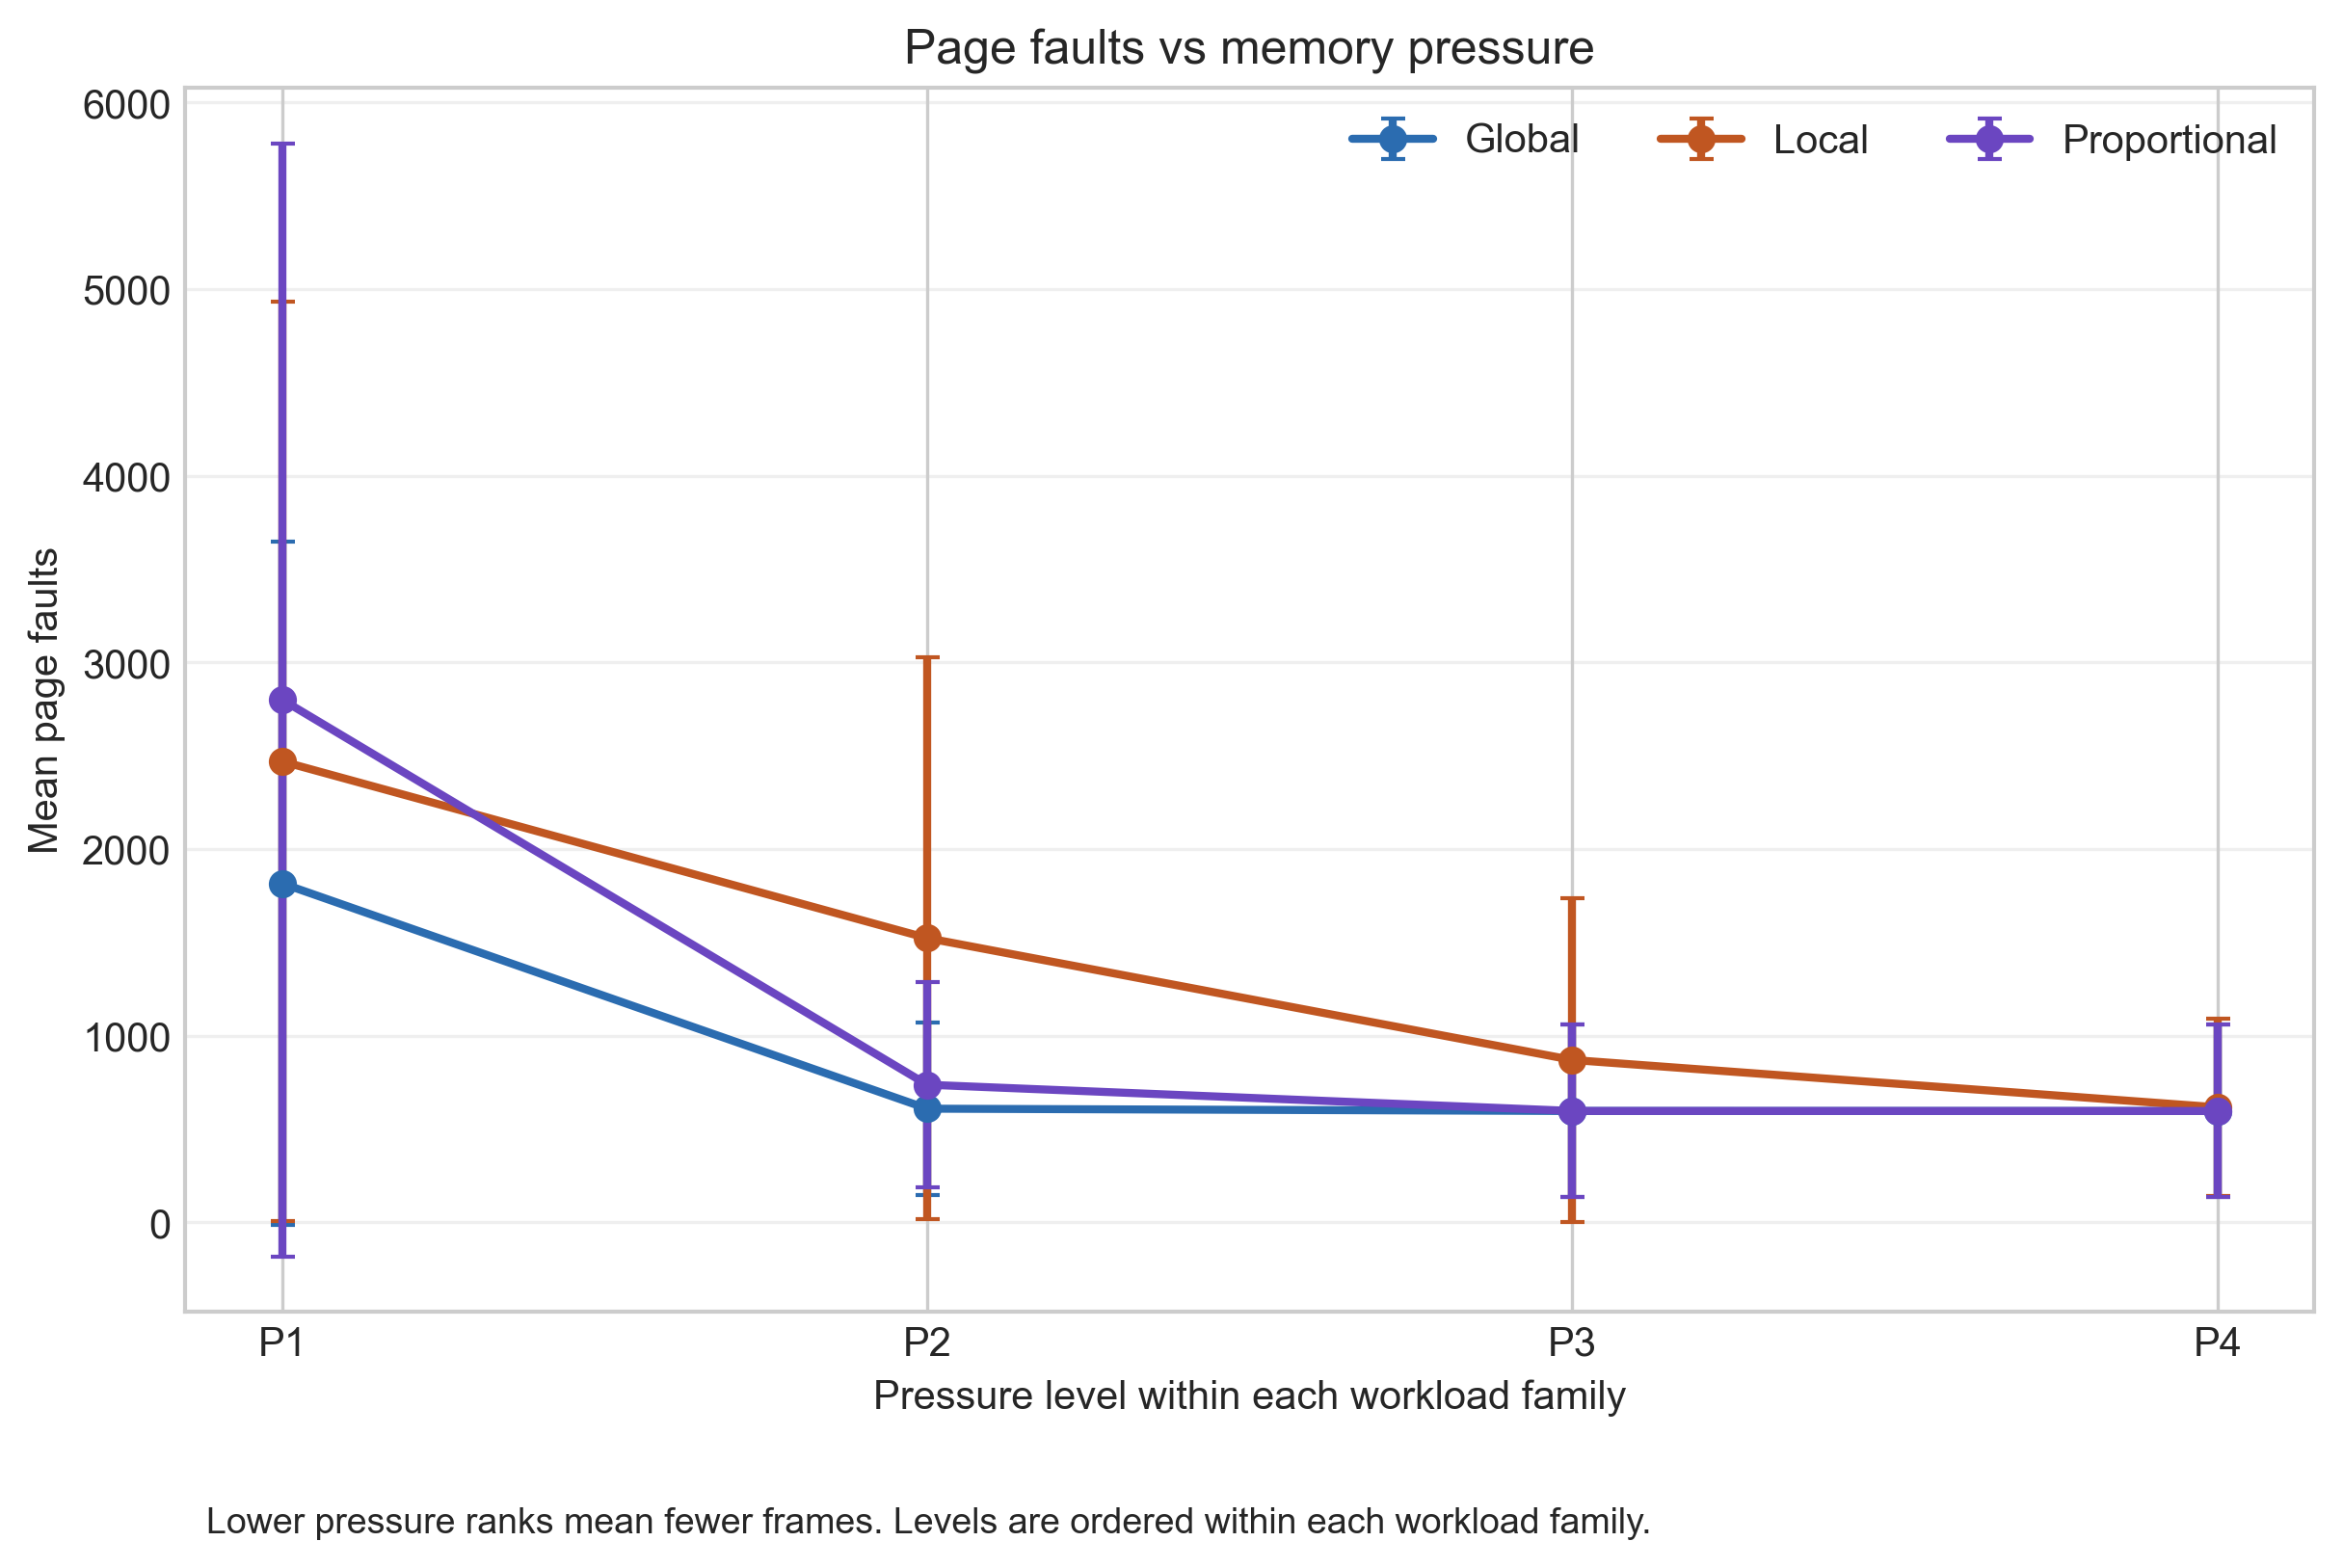
\includegraphics[width=\linewidth]{results/figures/page_faults_vs_memory_pressure.png}
\caption{Page faults versus memory pressure in the final aggregate.}
\label{fig:pagefaults}
\end{figure}

Figure~\ref{fig:pagefaults} shows the expected pressure effect: tighter memory budgets increase fault sensitivity. The exact policy ranking varies by workload, but the high-level pattern is stable enough to support the conclusion that fault minimization is not the same as fairness optimization.

\textbf{Interpretation.} FIFO evicts the oldest resident page without using recency history, and global allocation lets any process draw from the entire frame pool. In this campaign, that combination often reduced aggregate faults because bursty processes were not constrained by fixed local quotas. The same flexibility can be unfair: a process with a larger working set or a more aggressive reference stream can occupy frames that would otherwise protect another process. NRU with local or proportional allocation reduced the selected worst-case slowdown rows because those allocation regimes bound cross-process interference.

\subsection{Trace-Driven Results}
Table~\ref{tab:trace_best} summarizes the trace-driven replay results. The trace rows are much smaller than the synthetic matrix, but they are valuable because they verify that the same tooling can replay concrete event streams. FIFO with global allocation again produced the table-selected lowest page-fault counts in the trace rows, while FIFO with proportional allocation minimized worst-case slowdown across the five trace rows. Jain's-index winners still varied by trace, reinforcing the need to report more than one metric.

\begin{table}[t]
\centering
\small
\caption{Headline results by trace workload.}
\label{tab:trace_best}
\resizebox{\linewidth}{!}{%
\begin{tabular}{llll}
\toprule
Trace workload & Lowest page faults & Lowest worst slowdown & Highest Jain's index \\
\midrule
report\_locality\_heavy & FIFO + GlobalAllocation (4.0) & FIFO + ProportionalAllocation (1.0782) & NRU + GlobalAllocation (0.99867) \\
report\_mixed\_heterogeneous & FIFO + GlobalAllocation (11.0) & FIFO + ProportionalAllocation (0.9630) & SecondChance + GlobalAllocation (0.99846) \\
report\_streaming\_sequential & FIFO + GlobalAllocation (16.0) & FIFO + ProportionalAllocation (1.0486) & SecondChance + GlobalAllocation (0.99965) \\
report\_thrashing\_pressure & FIFO + GlobalAllocation (10.0) & FIFO + ProportionalAllocation (1.0739) & WSClock + LocalAllocation (0.99963) \\
sample\_trace & FIFO + GlobalAllocation (5.0) & FIFO + ProportionalAllocation (0.9342) & LRU + LocalAllocation (0.99781) \\
\bottomrule
\end{tabular}%
}
\end{table}

\begin{figure}[t]
\centering
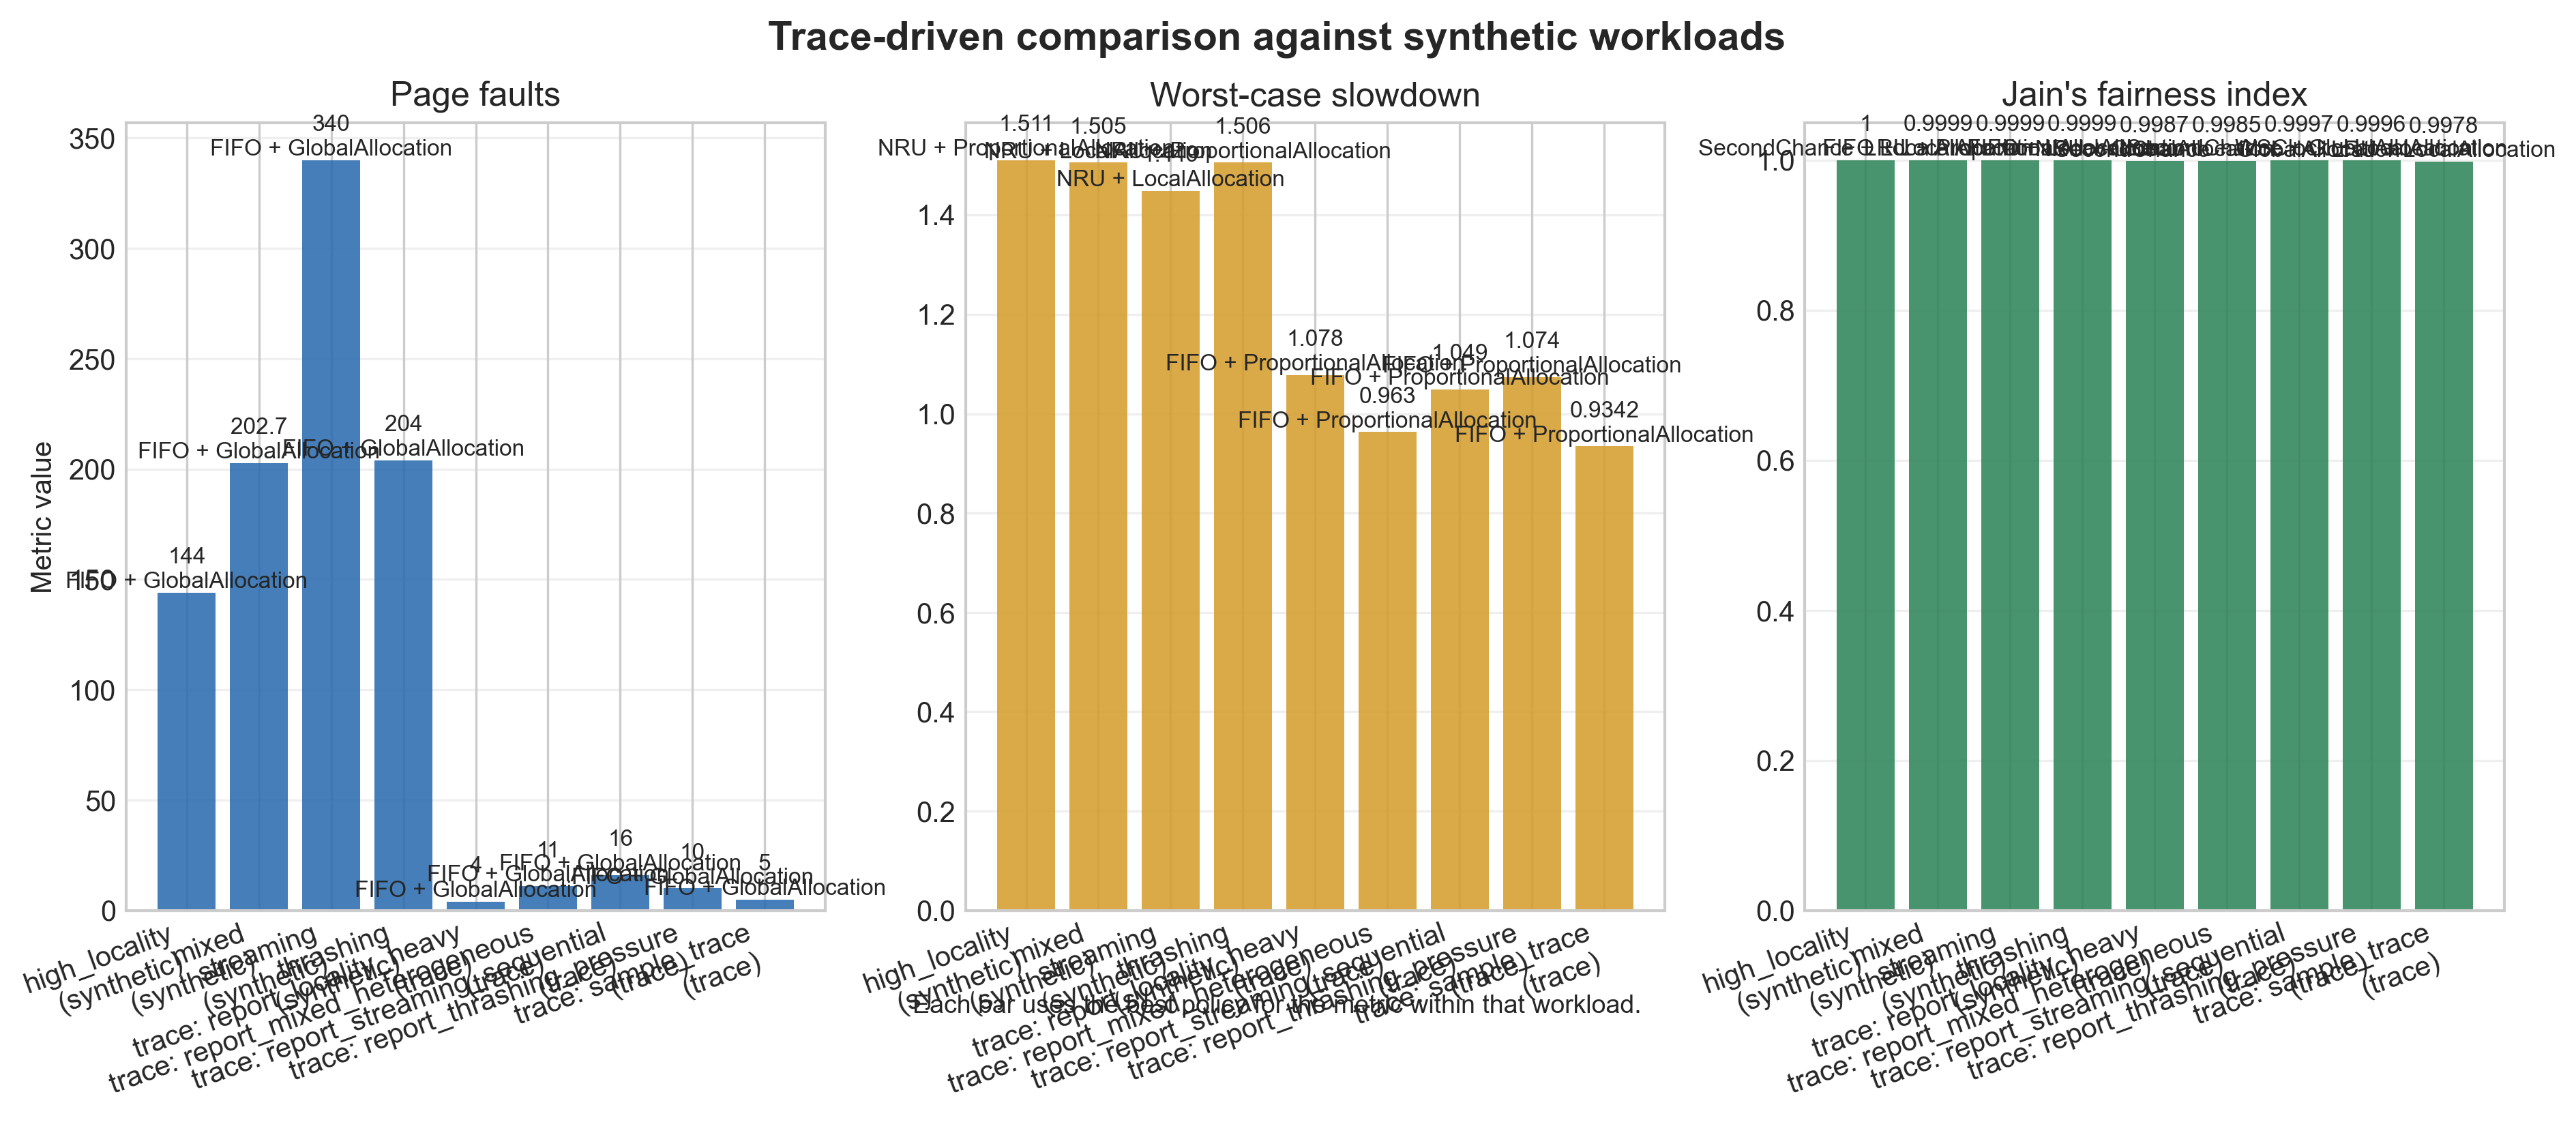
\includegraphics[width=\linewidth]{results/figures/trace_driven_comparison.png}
\caption{Trace-driven comparison across report-grade trace families.}
\label{fig:tracecompare}
\end{figure}

\textbf{Interpretation.} Trace-driven trends largely match synthetic trends for the page-fault winner: FIFO + Global remains the most efficient combination in terms of raw faults. For tail slowdown, proportional allocation is selected in all five trace rows. The differences are in magnitude: trace-driven faults are lower because the traces are shorter and more focused than the long synthetic sequences. This agreement across workload sources increases confidence that the main fault-versus-fairness tension is not solely an artifact of the synthetic workload generator.

\subsection{Efficiency vs.\ Fairness Trade-offs}
Figures~\ref{fig:worstslowdown} and~\ref{fig:jains} show that allocation policy changes the fairness story. Worst-case slowdown exposes tail behavior that average faults can hide, while Jain's index captures how evenly service is distributed. A policy that wins on faults can still create a worse slowest process, especially near the working-set boundary.

\begin{figure}[t]
\centering
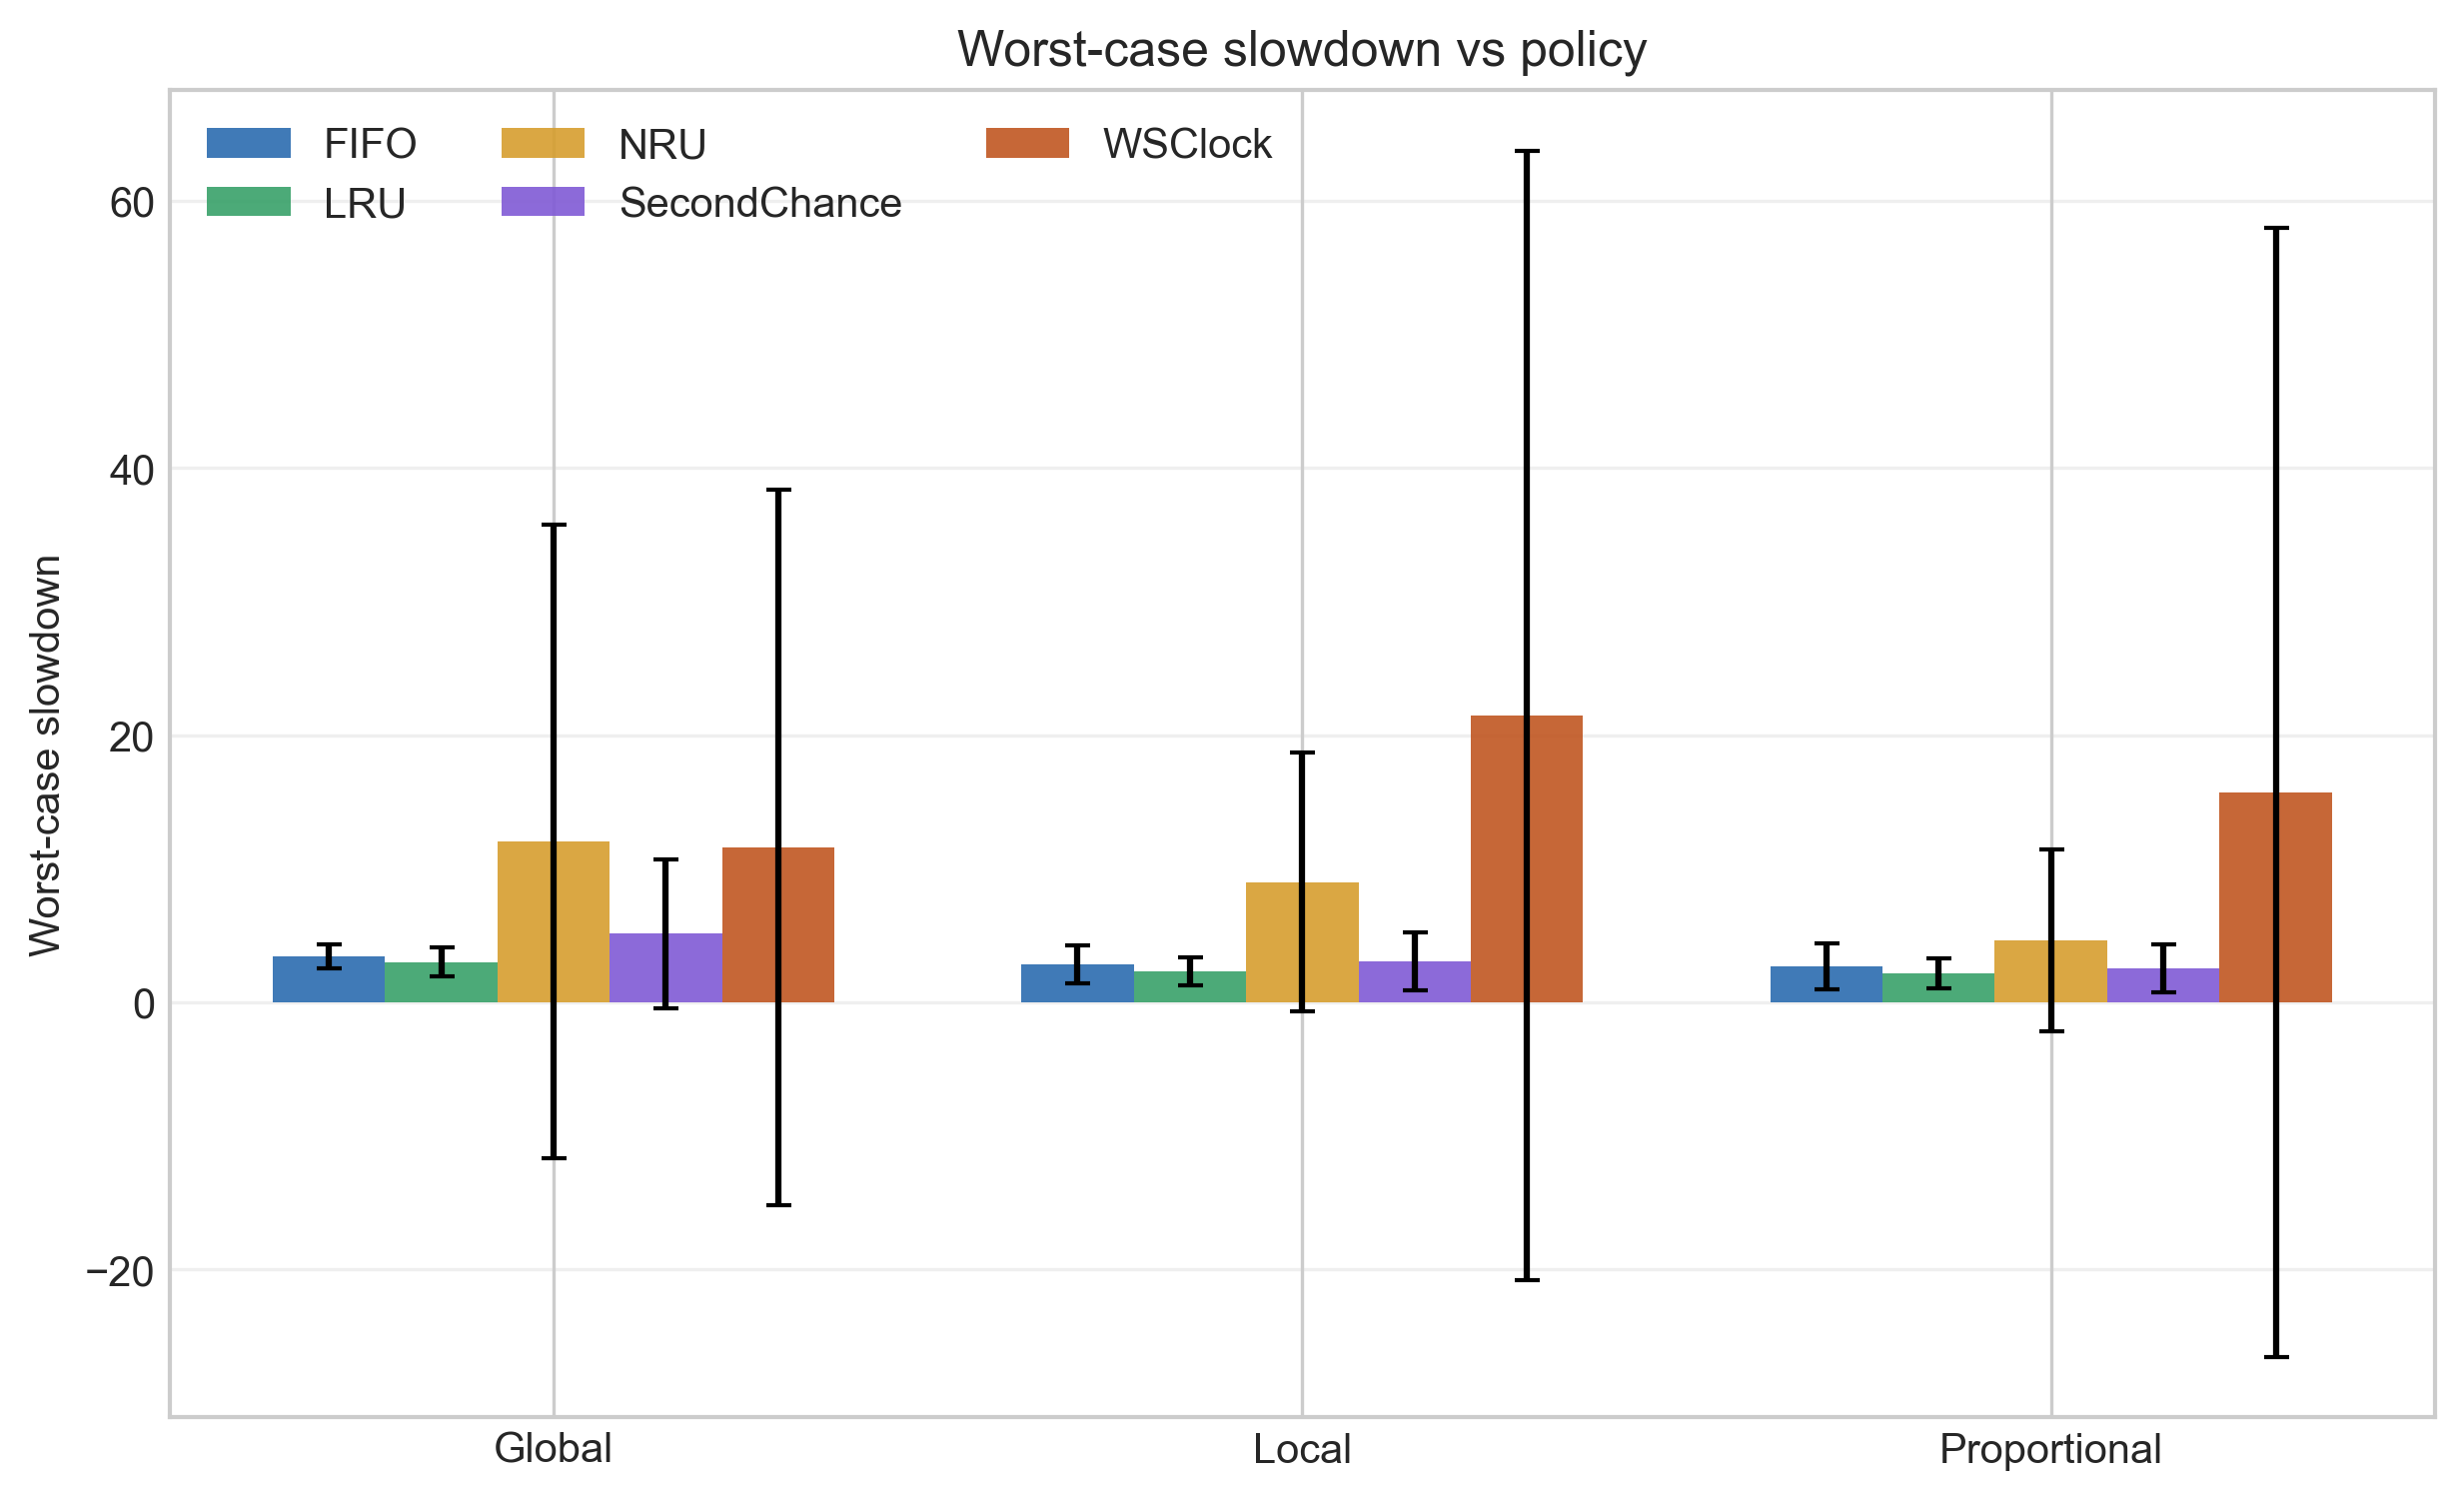
\includegraphics[width=\linewidth]{results/figures/worst_case_slowdown_vs_policy.png}
\caption{Worst-case slowdown by allocation policy in the final aggregate.}
\label{fig:worstslowdown}
\end{figure}

\begin{figure}[t]
\centering
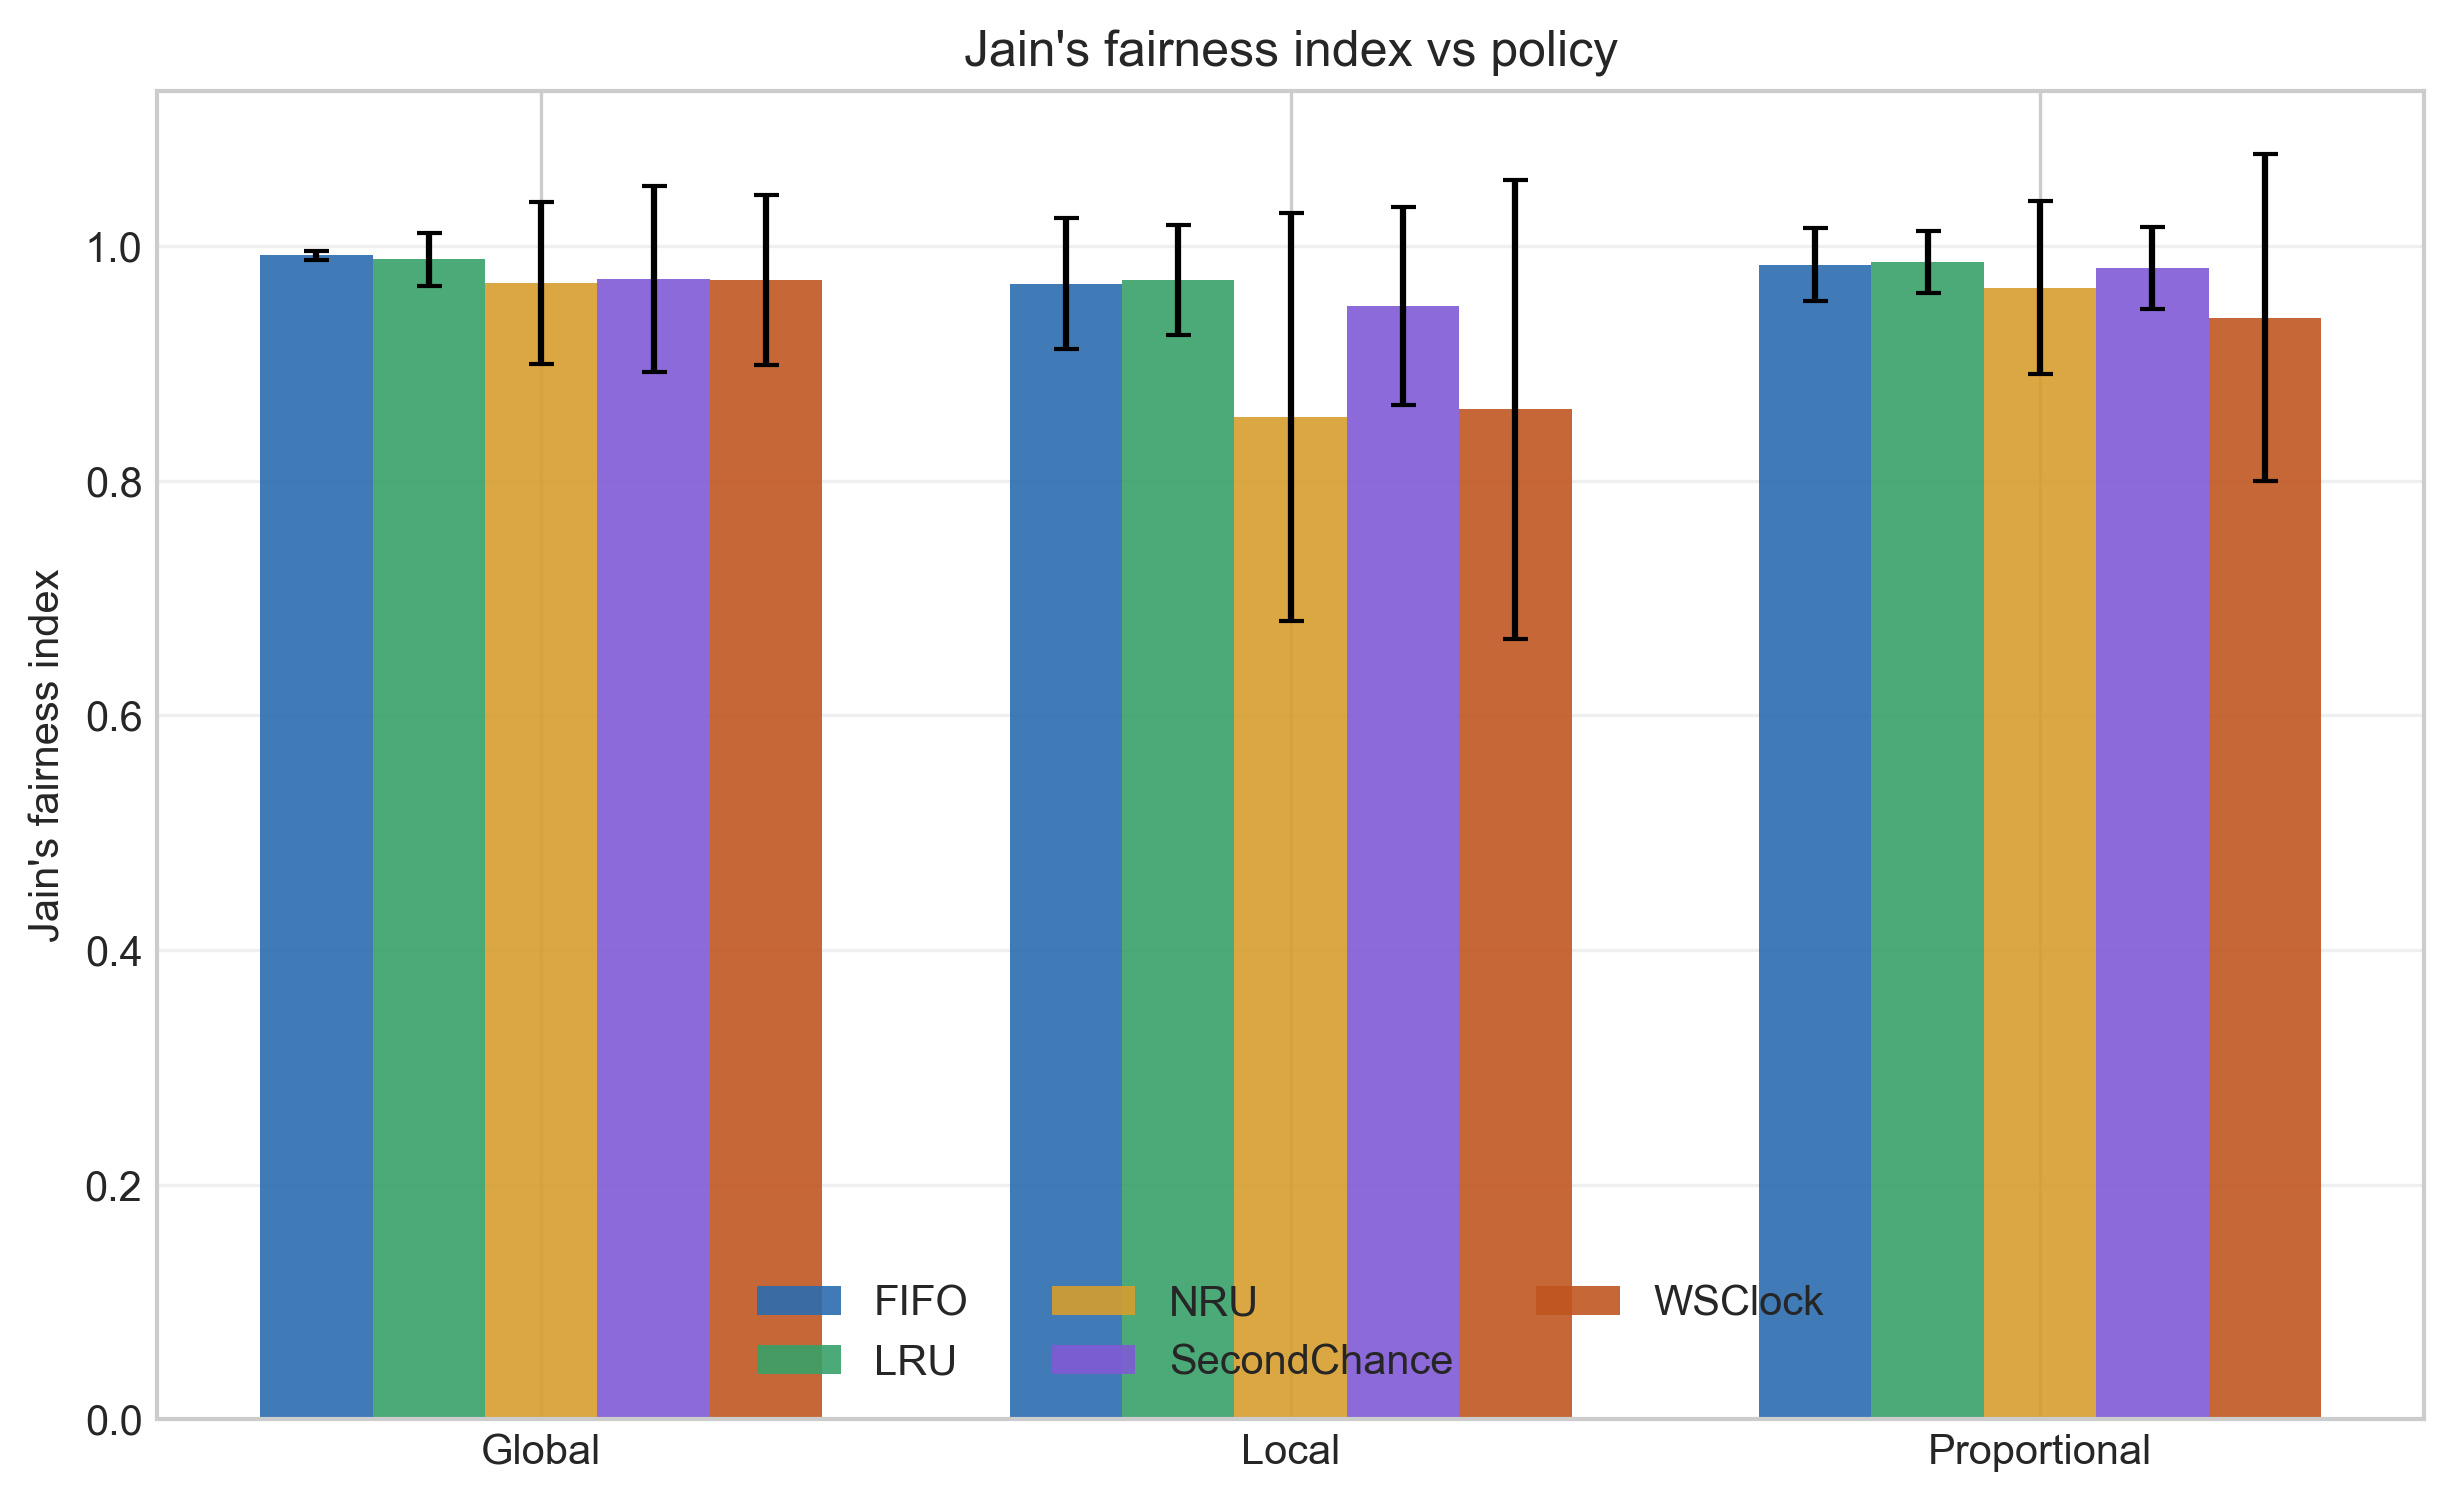
\includegraphics[width=\linewidth]{results/figures/jains_fairness_vs_policy.png}
\caption{Jain's fairness index by allocation policy in the final aggregate.}
\label{fig:jains}
\end{figure}

\textbf{Interpretation.} Near 1.0x--1.2x aggregate WSS, global allocation can let the most aggressive process capture a disproportionate share of frames. Local allocation prevents this by enforcing per-process limits, but those limits can be too rigid if one process has a genuinely larger working set. Proportional allocation attempts to balance the two: it divides frames by estimated demand, so no process is starved, yet some flexibility remains. In the report tables, proportional allocation is repeatedly selected for tail-slowdown or Jain's-index wins, making it the strongest compromise policy in this artifact.

\begin{table}[t]
\centering
\scriptsize
\caption{Final H1/H2/H3 hypothesis summary.}
\label{tab:hypothesis_summary}
\resizebox{\linewidth}{!}{%
\begin{tabular}{p{0.10\linewidth}p{0.31\linewidth}p{0.21\linewidth}p{0.14\linewidth}p{0.12\linewidth}}
\toprule
Hyp. & Test condition & Baseline $\rightarrow$ cmp. & Change & Status \\
\midrule
H1 & High locality, 4 procs, near 1.2x WSS & 326.2 $\rightarrow$ 325.1 faults & -0.34\% & Supported \\
H2 & Aggregate-WSS boundary, 4 procs & 0.01190 $\rightarrow$ 0.01886 variance & +58.53\% & Supported \\
H3 & Mixed workload, 4 procs, near WSS & 2.6449 $\rightarrow$ 3.2209 slowdown & +21.78\% & Not supported \\
\bottomrule
\end{tabular}}
\end{table}

\subsection{Runtime and Stability Observations}
The slowdown metrics are useful for directional fairness comparisons, but they are noisier than page faults. The isolation baseline study in \file{docs/isolation\_stability.md} reports 264 baseline groups, with 81 stable groups, 39 review groups, and 144 unstable groups. The median CV was 0.128607 and the mean CV was 0.1902, so the report treats exact slowdown magnitudes cautiously. This caveat does not invalidate the page-fault trends, and it is why the discussion emphasizes broad fairness patterns and hypothesis directions rather than single-run wall-clock values.

\section{Hypothesis Outcome Discussion}
\textbf{H1 is supported.} The H1 comparison used high-locality workloads with four processes near 1.2x aggregate WSS. LRU with global allocation reduced page faults from 326.2 to 325.1 compared with LRU local allocation, a 0.34\% reduction, while worst-case slowdown increased from 1.6298 to 3.6517, a 124.05\% increase. Jain's index also dropped from 0.99645 to 0.95621 in that slice. The fault improvement is small, but the slowdown penalty is large, confirming the expected efficiency--fairness trade-off.

\textbf{H2 is supported.} Near the aggregate WSS boundary with four processes, slowdown variance increased from 0.01190 under local allocation to 0.01886 under global allocation, a 58.53\% increase. This supports the hypothesis that global allocation can amplify fairness differences near the working-set boundary.

\textbf{H3 is not supported.} For the mixed workload with four processes near aggregate WSS, the FIFO/NRU local comparison condition increased worst-case slowdown from 2.6449 to 3.2209, a 21.78\% increase, instead of reducing it. The comparison condition also moved page faults from 1115.7 to 345.5, a 69.03\% reduction, so the data again show a fault/fairness divergence. Because the primary fairness metric did not improve, the result rejects the claim that simple local policies were better for fairness under the mixed-workload conditions tested.

\textbf{Implications.} The supported hypotheses show that memory pressure near the WSS boundary is the regime where fairness matters most. Operating-system designers should therefore be wary of global allocation when aggregate demand approaches physical memory size. The unsupported H3 suggests that the choice between simple and advanced policies is more nuanced than ``simpler is fairer''; the workload mix and allocation regime both matter.

\section{Threats to Validity}
The following threats limit the scope of the conclusions.

\textbf{Wall-clock timing noise.} Shared and isolated runtimes are measured on a general-purpose host, so operating-system scheduling and background activity can affect slowdown values even with quiet and pinned wrappers. The high coefficient of variation in some isolation baselines confirms this noise.

\textbf{Trace diversity.} The trace-driven study covers five report traces, which is enough to exercise replay support but not enough to represent the full range of real production workloads. The synthetic workloads are designed to stress specific behaviors, but they cannot capture every real-world access pattern.

\textbf{Simulator-to-kernel gap.} The simulator gives strong control over policies and instrumentation, but it omits many production details such as hardware prefetching, TLB behavior, disk scheduling, NUMA effects, and kernel paging heuristics. Conclusions are therefore strongest for comparative trends, not for absolute magnitudes.

\textbf{Validation scope.} The canonical validation report confirms readable source groups, no duplicate configurations, and complete shared/isolation runtime-record coverage after process identifiers are normalized. Its remaining warnings are host-noise outliers. For that reason, fairness conclusions are stronger directionally than as exact slowdown magnitudes.

\textbf{Page size and workload normalization.} The simulator uses a fixed page size and normalizes workloads to the same aggregate WSS scale. Different page sizes or normalization choices could shift exact magnitudes, though comparative trends are likely to remain stable.

\section{Reproducibility}
The repository is structured so that the result bundle and the report can be regenerated from the checked-in scripts. After installing dependencies from \file{requirements.txt}, the setup test is \texttt{python -m unittest discover}. The final matrix is launched through \file{experiments/run\_all\_experiments.py} with the \texttt{--final} option, and report tables and figures are regenerated by \file{scripts/build\_final\_report\_artifacts.py}. Windows users can run controlled timing experiments through \file{scripts/run\_quiet\_benchmark.ps1}; Unix-like environments can use the matching shell wrapper. The checked-in \file{README.md} and \file{docs/RESULTS\_BUNDLE.md} give the complete command list and artifact layout.

\section{Future Work}
Future work will focus on broadening the trace set, improving runtime isolation, and adding an explicit efficiency cost model. A useful next step is a weighted cost function that combines page faults, disk reads, disk writes, replacement activity, and slowdown penalties. This would let future experiments compare whether the policy that minimizes faults also minimizes total execution cost under more realistic storage-cost assumptions.

Additional directions include integrating TLB modeling into the simulator, exploring adaptive allocation policies that resize partitions at runtime, and evaluating the impact of page coloring and NUMA placement on fairness. A larger trace library drawn from cloud workloads and scientific applications would strengthen external validity.

\section{Conclusion}
This report evaluated a custom virtual memory simulator and trace-driven benchmark framework for replacement and allocation policies under memory pressure. The final evidence shows that H1 is supported, H2 is supported, and H3 is not supported. The central implication is that page-fault minimization alone is an incomplete policy-selection criterion: allocation choices can shift fairness and worst-case slowdown even when fault counts improve. The most important next direction is a broader trace set paired with a more explicit efficiency cost model, so future evaluations can compare fault, I/O, runtime, and fairness costs in a single framework. This project makes a concrete, reproducible contribution to the course goal of understanding how operating-system memory-management decisions affect real system behavior.

\begin{thebibliography}{10}
\bibitem{Belady1966}
L.~A. Belady, ``A study of replacement algorithms for a virtual-storage computer,'' \emph{IBM Systems Journal}, vol.~5, no.~2, pp. 78--101, 1966.

\bibitem{Denning1968}
P.~J. Denning, ``The working set model for program behavior,'' \emph{Communications of the ACM}, vol.~11, no.~5, pp. 323--333, May 1968.

\bibitem{Denning1970}
P.~J. Denning, ``Virtual memory,'' \emph{Computing Surveys}, vol.~2, no.~3, pp. 153--189, Sept. 1970.

\bibitem{Silberschatz2019}
A. Silberschatz, P.~B. Galvin, and G. Gagne, \emph{Operating System Concepts}, 10th~ed.\hskip 1em plus 0.5em minus 0.4em\relax Hoboken, NJ, USA: Wiley, 2019.

\bibitem{Ghandeharizadeh2015}
S. Ghandeharizadeh, S. Irani, and J. Lam, ``Cache replacement with memory allocation,'' in \emph{Proc. of the Meeting on Algorithm Engineering and Experiments}.\hskip 1em plus 0.5em minus 0.4em\relax SIAM, 2015, pp. 15--28.

\bibitem{Basu2013}
A. Basu, J. Gandhi, J. Chang, M.~D. Hill, and M.~M. Swift, ``Efficient virtual memory for big memory servers,'' in \emph{Proc. of the 40th Annual Int. Symp. on Computer Architecture (ISCA)}.\hskip 1em plus 0.5em minus 0.4em\relax ACM, 2013, pp. 237--248.

\bibitem{Park2022}
C.~H. Park, I. Vougioukas, A. Sandberg, and D. Black-Schaffer, ``Every walk's a hit: Making page walks single-access cache hits,'' in \emph{Proc. of the 27th ACM Int. Conf. on Architectural Support for Programming Languages and Operating Systems (ASPLOS)}, 2022, pp. 1--14.

\bibitem{Powers2019}
B. Powers, D. Tench, E.~D. Berger, and A. McGregor, ``Mesh: Compacting memory management for {C/C++} applications,'' in \emph{Proc. of the 40th ACM SIGPLAN Conf. on Programming Language Design and Implementation (PLDI)}.\hskip 1em plus 0.5em minus 0.4em\relax ACM, 2019, pp. 333--346.

\bibitem{Mytkowicz2009}
T. Mytkowicz, A. Diwan, M. Hauswirth, and P.~F. Sweeney, ``Producing wrong data without doing anything obviously wrong!'' in \emph{Proc. of the 14th Int. Conf. on Architectural Support for Programming Languages and Operating Systems (ASPLOS)}.\hskip 1em plus 0.5em minus 0.4em\relax ACM, 2009, pp. 265--276.

\bibitem{Schwalb2015}
D. Schwalb, T. Berning, M. Faust, M. Dreseler, and H. Plattner, ``{nvm malloc}: Memory allocation for {NVRAM},'' in \emph{Proc. of the 6th Int. Workshop on Accelerating Data Management Systems using Modern Hardware and Infrastructures (ADMS)}.\hskip 1em plus 0.5em minus 0.4em\relax 2015, pp. 61--72.
\end{thebibliography}

\end{document}
